\documentclass[]{article}

%%use packages%%
\usepackage[utf8]{inputenc}
\usepackage[english]{babel}
\usepackage[export]{adjustbox}
\usepackage{lipsum}
\usepackage{titlesec}
\usepackage{lmodern}
\usepackage{titling}
\usepackage{amssymb,amsmath}
\usepackage{ifxetex,ifluatex}
\usepackage{multicol}
\usepackage[a4paper, total={6in, 9in}]{geometry} %margin
\usepackage{fixltx2e} % provides \textsubscript
\usepackage{listings}
\usepackage{color}
\usepackage{caption}
\usepackage[]{microtype}
\usepackage{graphicx}
\usepackage{wrapfig}
\graphicspath{ {images/}}

\setlength{\columnsep}{0.7cm}

% use microtype if available
\IfFileExists{microtype.sty}{%

\UseMicrotypeSet[protrusion]{basicmath} % disable protrusion for tt fonts
}{}
\PassOptionsToPackage{hyphens}{url} % url is loaded by hyperref
\usepackage{xcolor}
\usepackage[colorlinks = true,
linkcolor = blue,
urlcolor  = blue,
citecolor = blue,
anchorcolor = blue]{hyperref}
\hypersetup{linkcolor=black}
\newcommand{\MYhref}[3][blue]{\href{#2}{\color{#1}{#3}}}%
\hypersetup{
            pdfborder={0 0 0},
            breaklinks=true}
\urlstyle{same}  % don't use monospace font for urls

%define subtitle
\newcommand{\subtitle}[1]{%
  \posttitle{%
    \par\end{center}
    \begin{center}\large#1\end{center}
    \vskip0.5em}%
}

%define indentations & sections spacing
\setlength{\parindent}{4em}
\titlespacing\section{0pt}{12pt plus 4pt minus 2pt}{0pt plus 4pt minus 2pt}

%%%%%%%%%%%%%%%%%%%%%%%%%%%%%%%%%%%%%%%%%%%%%%%%%%%%%%%
\begin{document}

\title{Understanding \& Developing Artificial Neural Networks}
\subtitle{Deerfield Academy Advance Computer Science Research}

\author{Yongyang (Neil) Nie}

\date{Feb, 2016}

\maketitle

\tableofcontents

\vspace{2.0cm}

%%%%%%%%%%%%%%%%%%%%%%%%%%%%%%%%%%%%%%%%%%%%%%%%%%%%%%%

\begin{multicols}{2}

\section{Abstract:}

Machine learning~is a subset of artificial intelligence \footnote{Artificial Intelligence A Modern Approach http://citeseerx.ist.psu.edu/viewdoc/download?doi=10.1.1.259.8854\&rep=rep1\&type=pdf} that provides
computers with the ability to learn without being explicitly
programmed. \footnote{ Samuel, Arthur L. (1959). "Some studies in machine learning using the game of checkers". IBM Journal of research and development.} Machine learning~focuses on the development of computer
programs that can change when exposed to new data.

There are many methods and algorithms for machine learning, from Support Vector
Machine\footnote{https://en.wikipedia.org/wiki/Support\_vector\_machine}
to Artificial Neural Networks\footnote{https://en.wikipedia.org/wiki/Artificial\_neural\_network}.
One of the common purpose for learning algorithms is to classify complex data. It can be used in analyzing human genetics and genomics. \footnote{Machine learning applications in genetics and genomics, Libbrecht, Maxwell W. http://dx.doi.org/10.1038/nrg3920}

%%%%%%%%%%%%%%%%%%%%%%%%%%%%%%%%%%%%%%%%%%%%%%%%%%%%%%%

\section{Introduction:}

	There are two types of machine learning, one is supervised machine
learning\footnote{Mehryar Mohri, Afshin Rostamizadeh, Ameet Talwalkar
  (2012)~\emph{Foundations of Machine Learning}, The MIT
  Press~\href{https://en.wikipedia.org/wiki/Special:BookSources/9780262018258}{ISBN
  9780262018258}.}. Supervised learning~is the~machine learning~task of
inferring a function from labeled training data. Each example is a pair consisting of an input object and a desired output value. By doing some calculation, the network can make rudimentary predictions and correct itself based on the training data to make more desired prediction. In this research, we will mainly focus on artificial neural networks and
supervised machine learning. 

This paper will discuss the principles behind designing, building, and
debugging an artificial neural network. All of the data are collect from a project I built that can recognize handwritten digits. The projects is written mainly in Objective-C and Python. You can find the resources on
\href{https://github.com/NeilNie/Neural-Network-Research}{Github}.

\subsection{What's neural networks}

\centerline{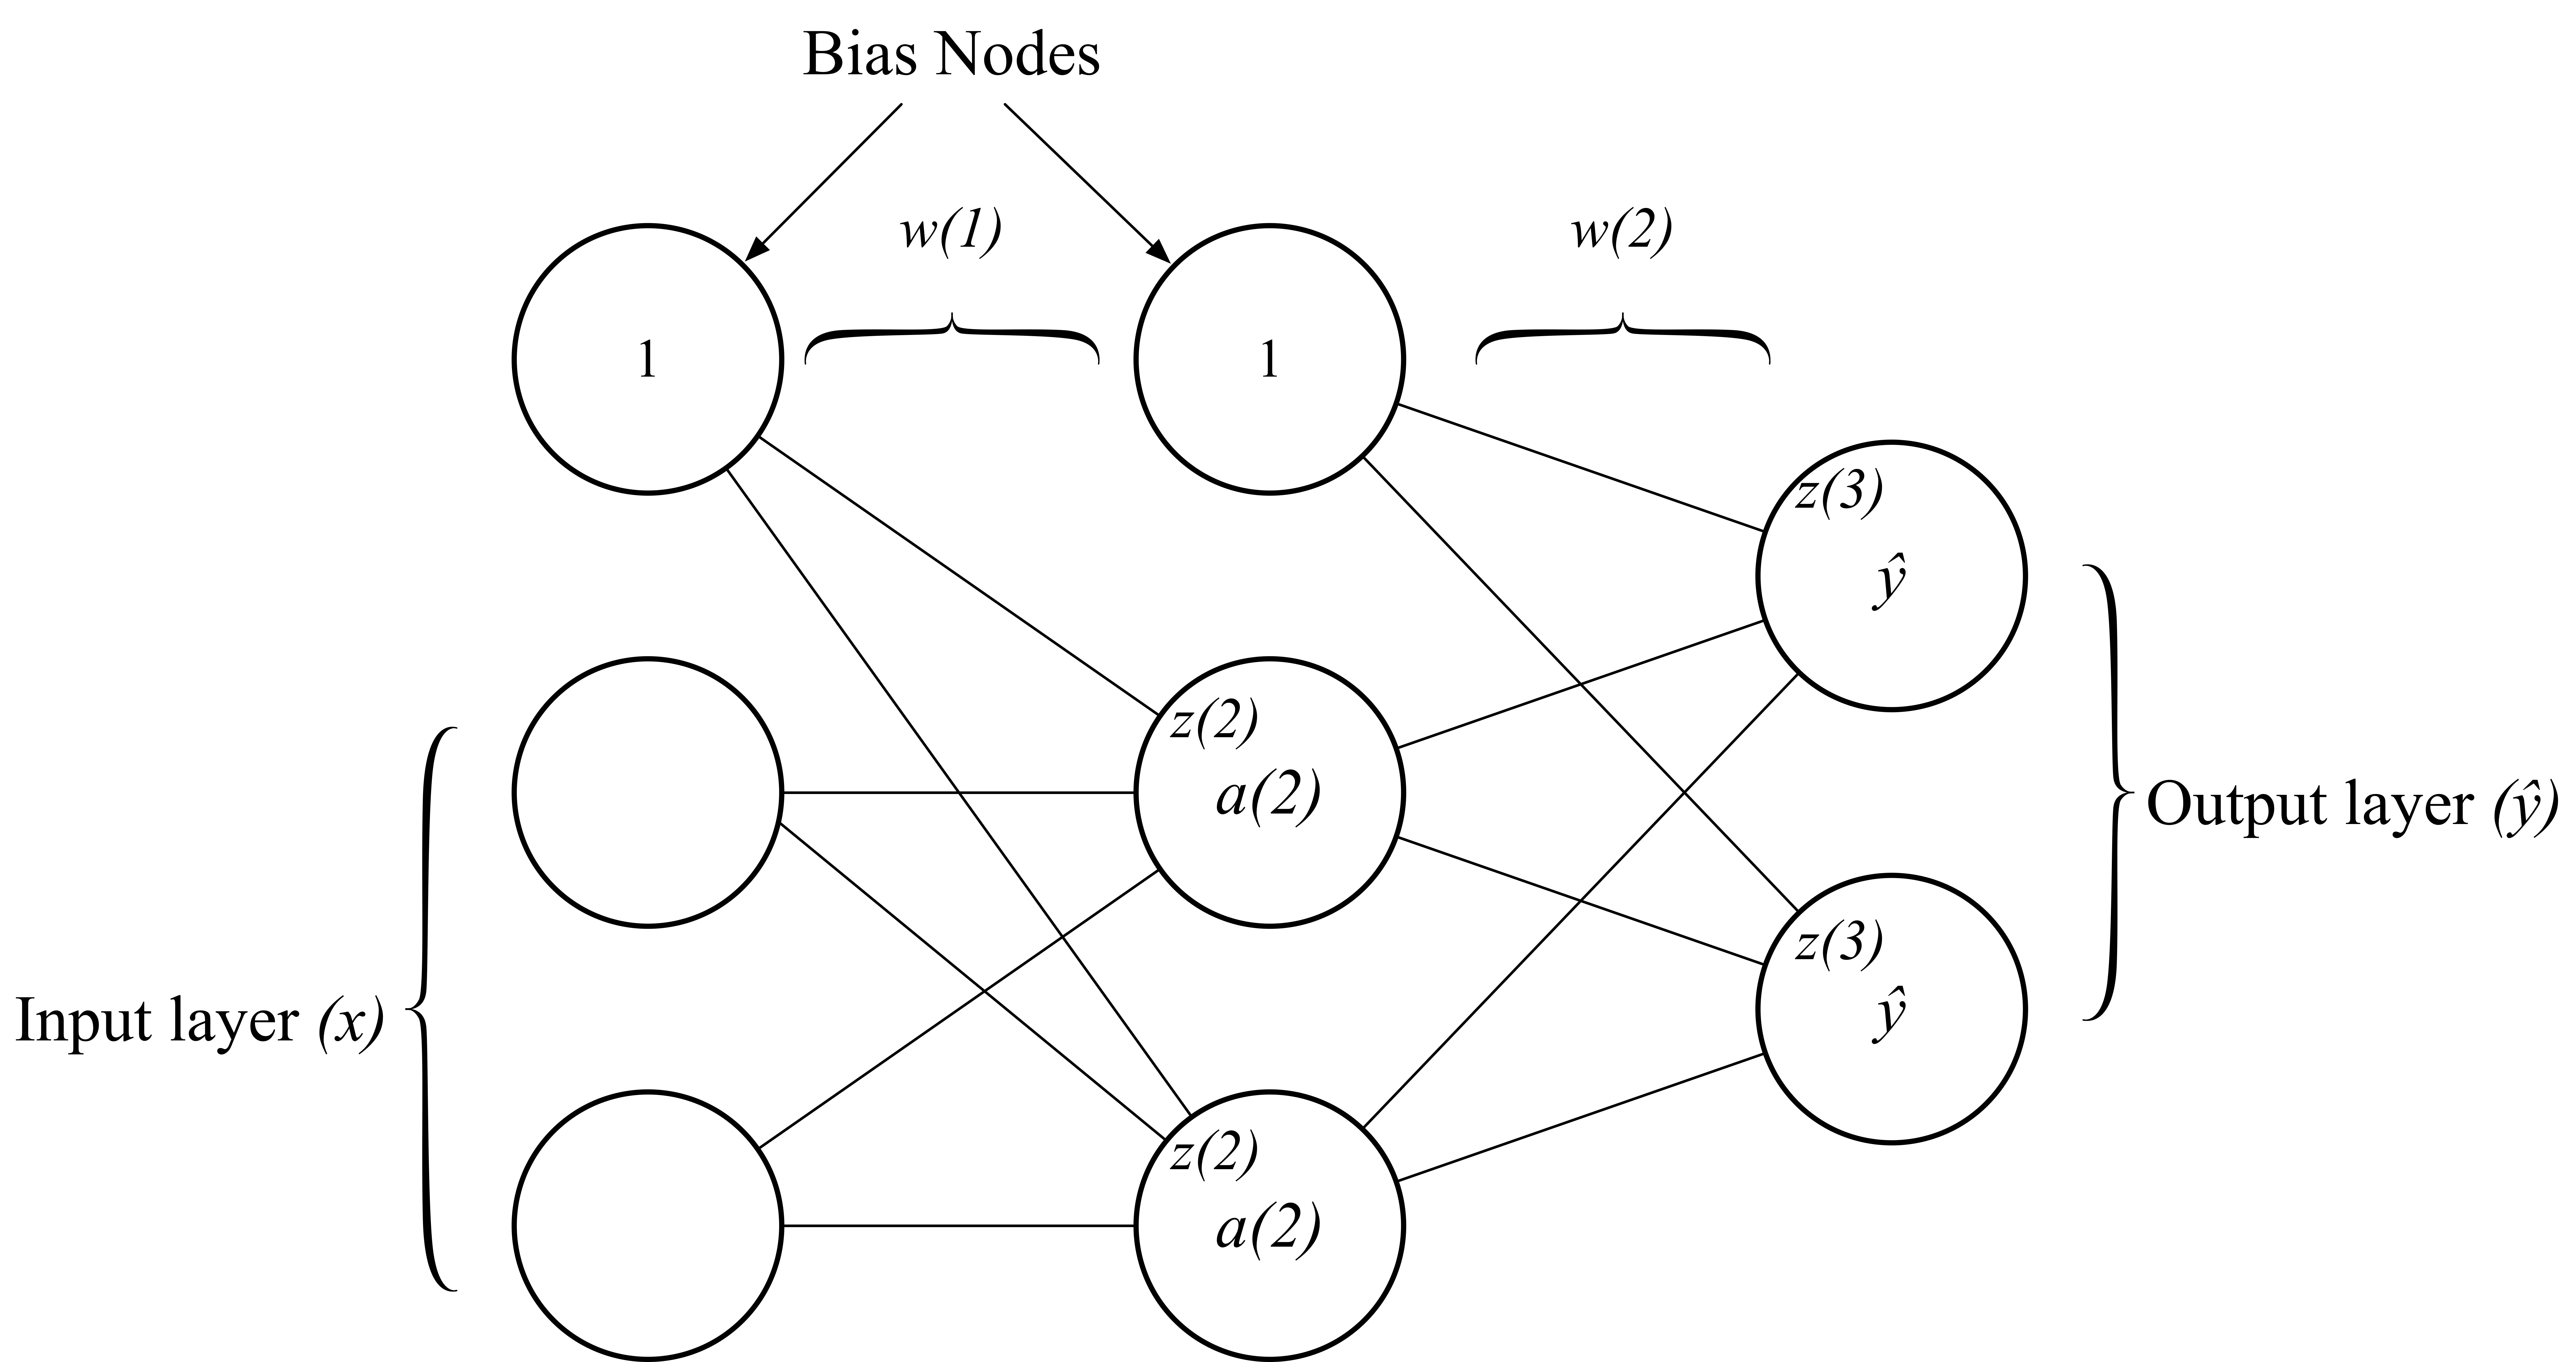
\includegraphics[width=1\linewidth]{nn} }
\centerline{Figure 1}
\vspace{0.5cm}

In the diagram above, you can find the important components in a neural network. First of all, most neural networks have a input and a output layer. Many neural networks will have hidden layer(s), when there numerous hidden layers, we consider that as deep learning \footnote{Deep learning Yann LeCun,	Yoshua Bengio \& Geoffrey Hinton http://dx.doi.org/10.1038/nature14539}, which is out of our scope. 

Secondly for neural networks in this paper, there are synapses connecting every node to every node in the next layer. All synapses have weights, a floating point number that will govern how the network behaves. Since the input is often static, the commonly used way to improve the prediction of a network is to modify the weights on synapses. 

Thirdly, there is one bias node connected to every layer in the network except the first layer. The bias will horizontally shift the activation function. This behavior will likely help the network learn more accurately. \footnote{Role of Bias in Neural  networks http://stackoverflow.com/questions/2480650/role-of-bias-in-neural-networks}

\subsection{Why neural networks}

Neural networks, with their remarkable ability to derive meaning from complicated or imprecise data, can be used to extract patterns and detect trends that are too complex to be noticed by either humans or other computer techniques. A trained neural network can be thought of as an "expert" in the category of information it has been given to analyze. \footnote{This section is reference from NEURAL NETWORKS 
	by Christos Stergiou and Dimitrios Siganos  https://www.doc.ic.ac.uk/~nd/surprise\_96/journal/vol4/cs11/report.html\#Why\%20use\%20neural\%20networks}

%%%%%%%%%%%%%%%%%%%%%%%%%%%%%%%%%%%%%%%%%%%%%%%%%%%%%%%

\section{Forward Feed:}

The neural network will begin be taking in some inputs and making some
predictions based on the inputs and the weights between nodes. We can
think of it like a one by two matrix. There will be a weight connecting
every input layer node to every output layer node, therefore, there are
six weights between the input layer and the second layer. The matrix
calculation should yield us some result

\[\begin{bmatrix}
a
\end{bmatrix}\ \lbrack w \rbrack = \begin{bmatrix}
z
\end{bmatrix}\]

If we give the matrices some names, call inputs \emph{x}, weights
\emph{w\textsubscript{(l)}} and output \emph{z\textsubscript{(l)}.} In
our case, \emph{l} indicate the layer, for example, the first layer
weights are \emph{w\textsubscript{(1)}}. \emph{z\textsubscript{(l)}}
represent the output matrix with layer \emph{l}, in this case, the
output z is the hidden layer output.

\begin{equation}
	\text{\ x}w_{\left( n \right)} = \ z_{(n)}\
\end{equation}

Afterwards, we have to apply an activation function\footnote{https://en.wikipedia.org/wiki/Activation\_function}.
The activation function that I used in this research and this paper will
be the sigmoid function. This is a complete cycle, there is one more
layer to go in order to yield a result. Note, in a multilayer neural
network, this process will be repeated until we yield some output. In
our case, we only have to do this twice. The activation function is
shown as below.

\[\sigma\left( z \right) = \ \frac{1}{1 + e^{- z}}\]
\begin{equation}
	{\text{\ a}}_{\left( 2 \right)} = f(z_{\left( 2 \right)})\
\end{equation}


By applying the same process as before, this time, the inputs will be
\emph{a\textsubscript{(2)} then, z\textsubscript{(3)}} will be our final
result. This process is known as forward feed. It's relatively
straightforward.

\[z_{\left( 3 \right)} = \ \text{\ a}_{\left( 2 \right)}w_{(2)}\]

After we yield some result, we can more on and look at how far off we
are from the expected result. We need some methods to quantify this and
so adjustments to the network to minimize error.

\begin{equation}
	\sigma'\left( z \right) = \ \sigma\left( z \right)(1 - \sigma(z))\
\end{equation}

\section{Quantifying and Minimizing Cost:}

Now the neural network can make calculation/predictions, however, the
result is far from desired. In almost all learning algorithms, the input
data cannot be altered, therefore the x term is constant in equation
one. In order to change the output \emph{z} the only option is to change
the weights \emph{w}.

First of all, we have to come up with ways to quantify the cost.

\begin{equation}
\left( 3 \right)\ C = \sum_{j}^{}{\frac{1}{2}{(\hat{y} - y)}^{2}}\
\end{equation}

C is the cost, which equals to the sum of all the differences between
calculated result and actual result squared and times one half. We can
take advantage of the equation derived above and substitute for some of
the variable.

\begin{equation}
	\ C = \ \sum_{J}^{}{\frac{1}{2}\left( y - f\left( f\left( xw_{\left( 1 \right)} \right)w_{\left( 2 \right)} \right) \right)^{2}}
\end{equation}


Here we have it, a way to quantify the cost of the neural network. This
function will be referred to as the cost function. Now, we have to solve
the problem, how do we minimize C, will brute force work? It turns out,
no, because in a three-node neural network we have to compute more than
a million possible weights, which will be gruesome.

We can think of the equation above as a function of cost in terms of all
possible weights. There will be one set of weights that will bring the
cost to the lowest. Then, this becomes a minimization problem.

\section{Gradient Descent:}

The best way to minimization the cost is to use gradient descent, a very
fast and classic way to solve problems like this. In fact, gradient
descent is widely used in math, image process and machine learning.

Gradient descent~is a~first-order~iterative~optimization~algorithm. To
find a~local minimum~of a function using gradient descent, one takes
steps proportional to the gradient (or of the
approximate gradient) of the function at the current point.

Gradient descent is also known as~steepest descent, or the~method of
steepest descent. The process can be seen as a ball rolling down a
hill\footnote{\url{https://iamtrask.github.io/2015/07/27/python-network-part2/}
  by Andrew}
and trying to find the lowest point. Note that actual physics doesn't
apply here and we will define our own movement of the ball.

\centerline{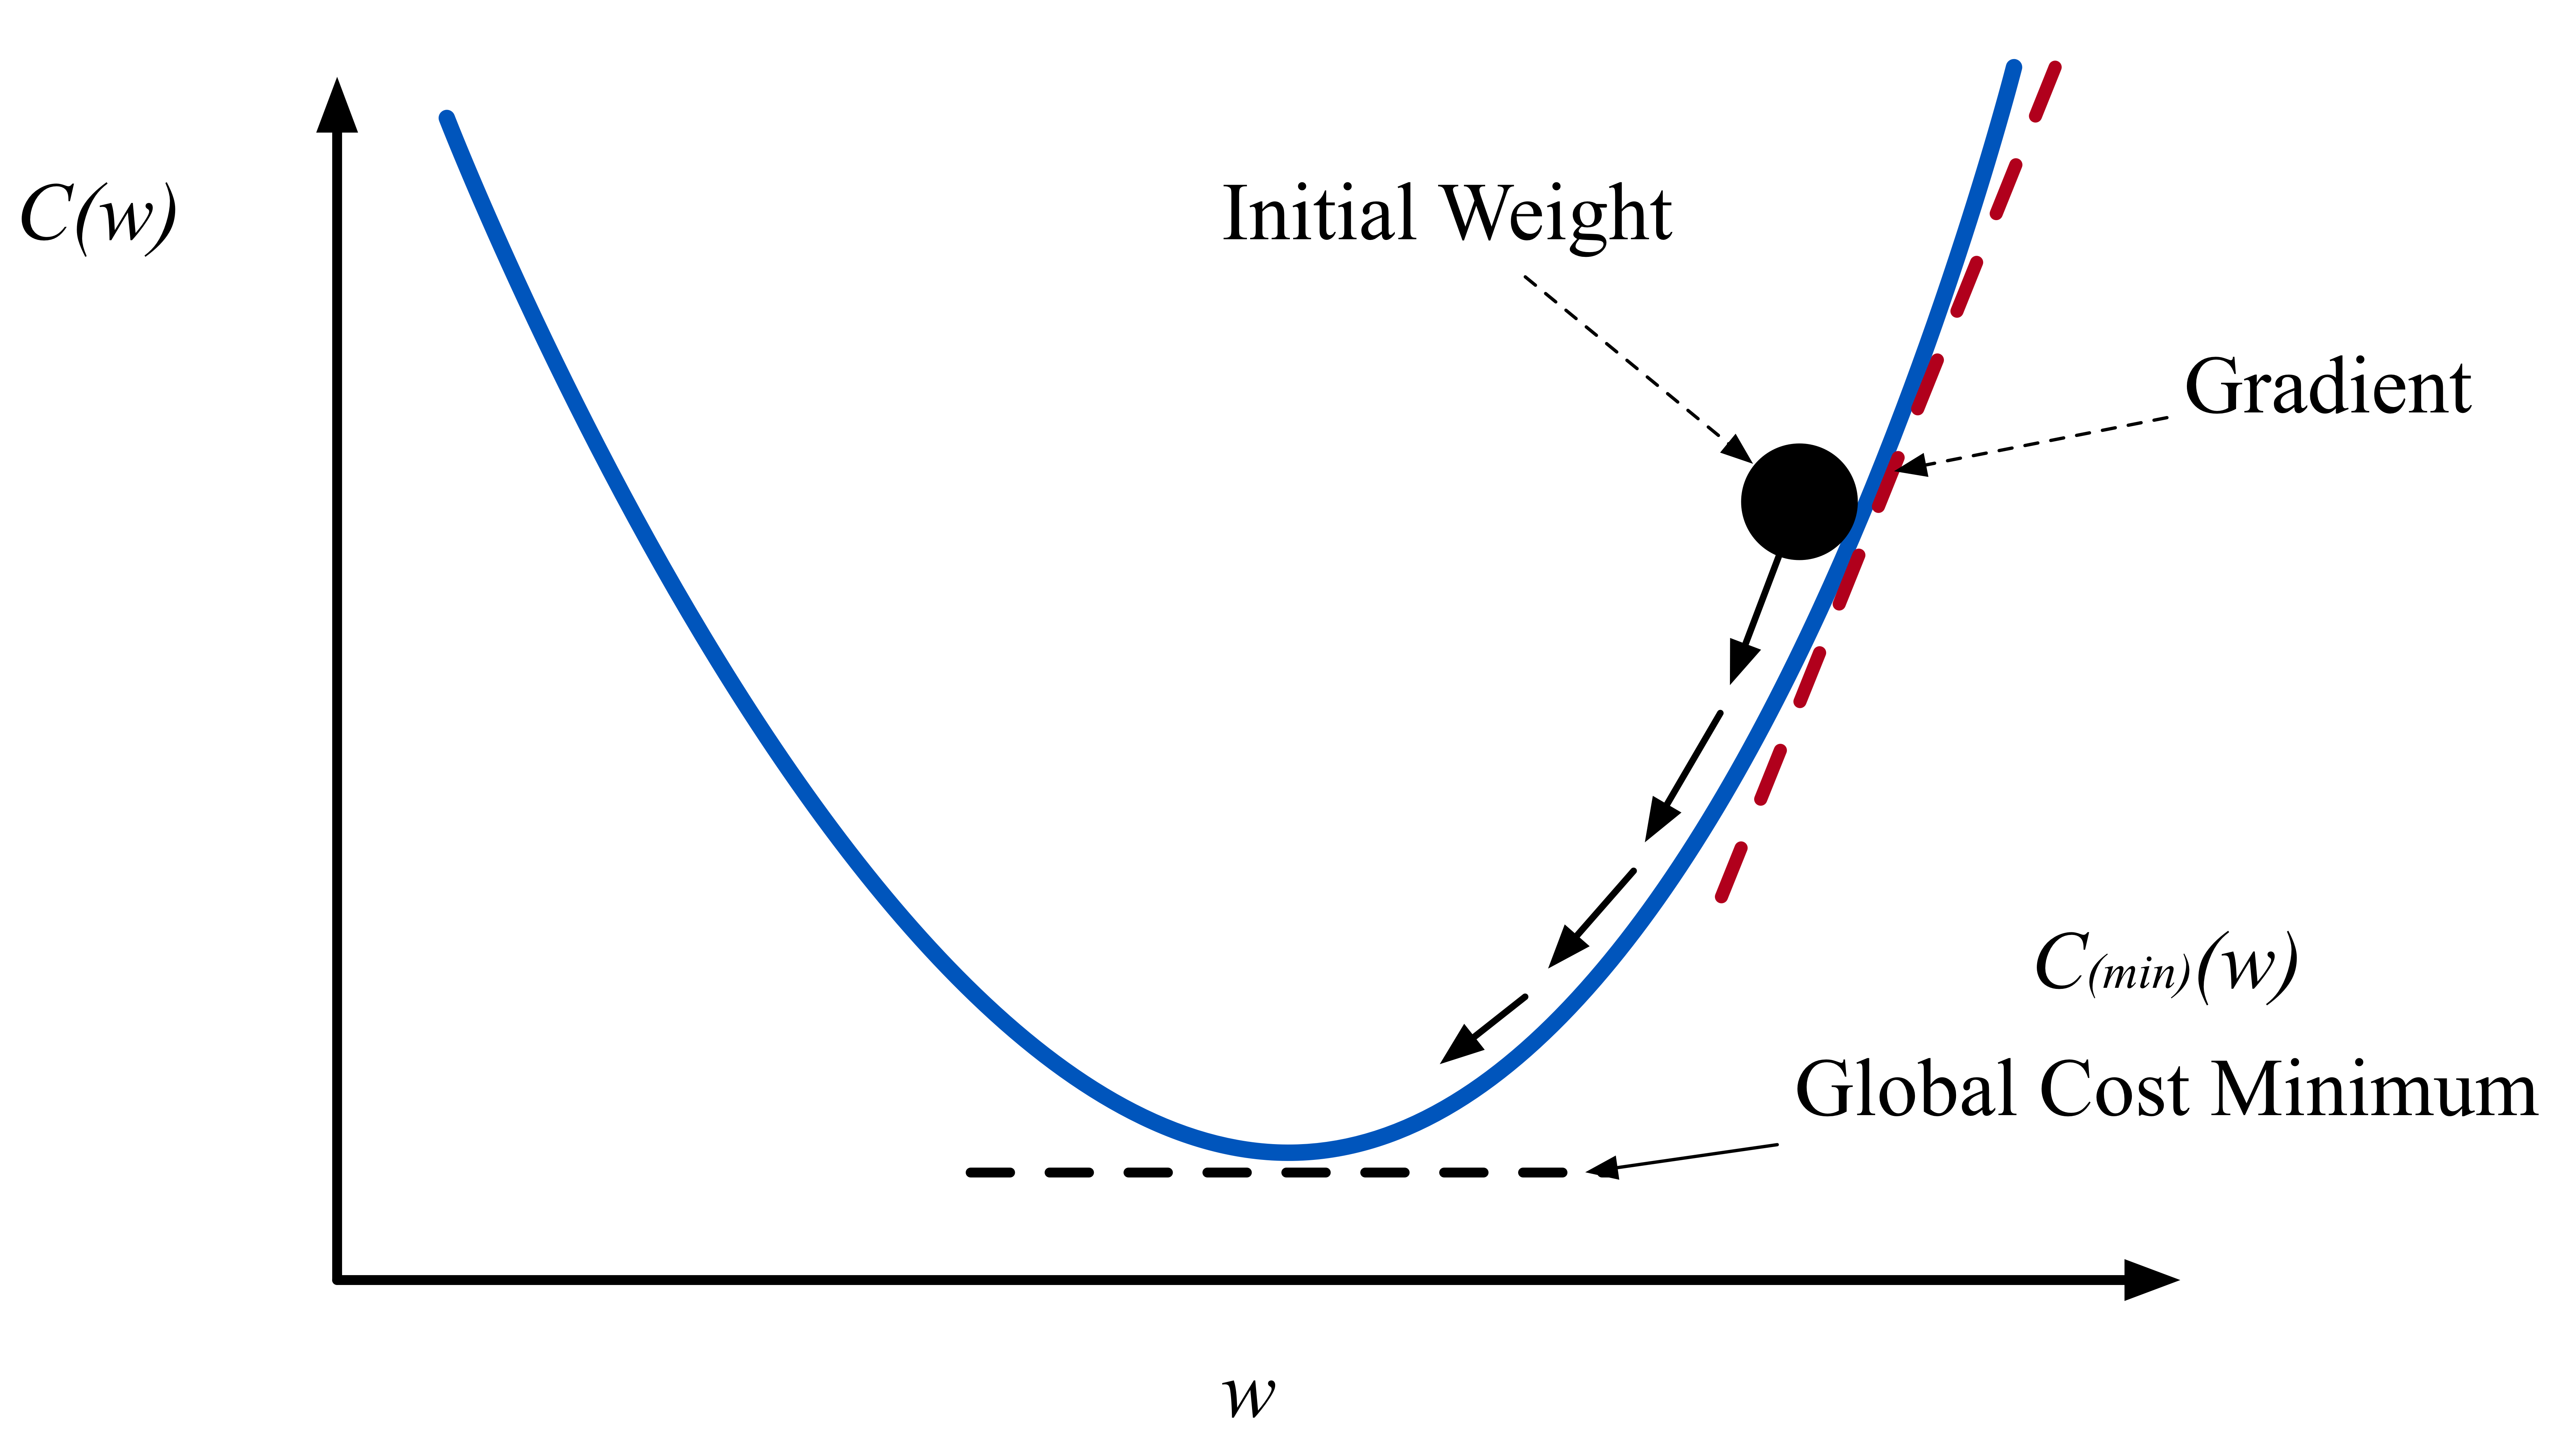
\includegraphics[width=1\linewidth]{gd} }
\centerline{Figure 2}
\vspace{0.5cm}

There are limitations to this method. First of all, what if we are stuck
in a local minimum, our goal is to find the global minimum for the cost
function. In another word, this method will not work properly for a non-convex
function. 

\centerline{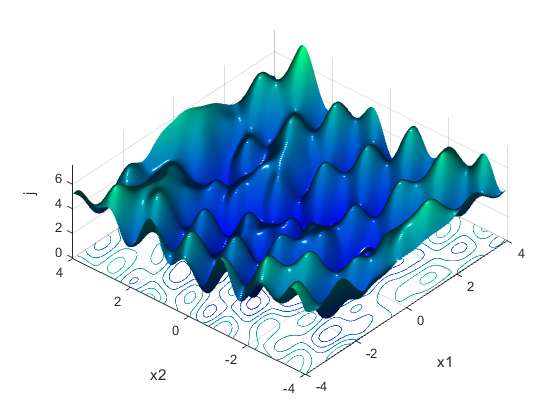
\includegraphics[width=0.9\linewidth]{non-convex} }
\centerline{Figure 3}
\vspace{0.5cm}

In fact, this problem is solved in equation (3), by squaring
the difference in \({(\hat{y} - y)}^{2}\), we are using the quadratic cost function, which is a convex function for any number of dimensions. 

\centerline{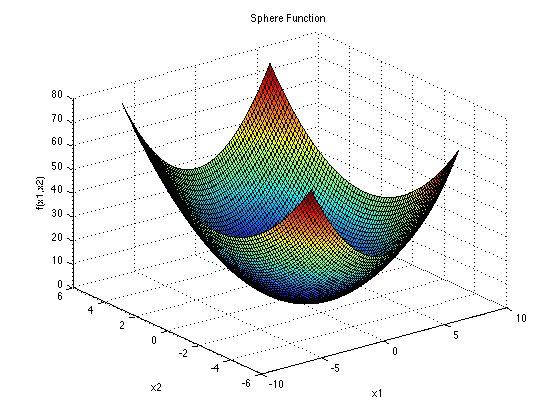
\includegraphics[width=0.9\linewidth]{convex} }
\centerline{Figure 4}
\vspace{0.5cm}

Thus, we can apply gradient descent without worrying about local minimums \footnote{Proof and definition of convex functions:
	http://mathworld.wolfram.com/ConvexFunction.html}. 

There are other types and variation of gradient descent as well. One of
the most commonly used one is Stochastic gradient descent~(SGD), also
known as~incremental~gradient descent, is a~stochastic approximation~of
the~gradient descent optimization method~for minimizing an~objective
function~that is written as a sum of~differentiable functions. In other
words, SGD tries to find minima or maxima by iteration. \footnote{\url{http://www.mit.edu/~dimitrib/Incremental_Survey_LIDS.pdf}
  Dimitri P. Bertsekas Report LIDS - 2848}

%%%%%%%%%%%%%%%%%%%%%%%%%%%%%%%%%%%%%%%%%%%%%%%%%%%%%%%

\section{Back propagation:}

With gradient descent, we can create a set of routines that can help us
to change the weights of the network to minimize the cost. This is call backprogation, which is the core of most of the  sophisticated learning algorithms. 

\subsection{Back propagation overview}

\emph{Phase 1: Propagation: Each propagation
involves the following steps:}
\footnote{The steps are referenced from
Wikipedia who referenced:
\href{http://numericinsight.com/uploads/A_Gentle_Introduction_to_Backpropagation.pdf}{A
Gentle Introduction to Backpropagation - An intuitive tutorial by
Shashi Sathyanarayana}~The article contains pseudocode ("Training
Wheels for Training Neural Networks") for implementing the algorithm.}  

\begin{enumerate}
\def\labelenumi{\arabic{enumi}.}
\item
  Forward propagation of a training pattern's input through the neural
  network in order to generate the network's output value(s).
\item
  Backward propagation of the propagation's output activations through
  the neural network using the training pattern target in order to
  generate the deltas (the difference between the targeted and actual
  output values) of all output and hidden neurons.
\end{enumerate}

\emph{
Phase 2: Weight update: For each weight, the following
steps must be
followed:}

\begin{enumerate}
\def\labelenumi{\arabic{enumi}.}
\item
  The weight's output delta and input activation are multiplied to find
  the gradient of the weight.
\item
  A ratio (percentage) of the weight's gradient is subtracted from the
  weight.
\end{enumerate}

\subsection{Mathematics behind backpropagation}

Backpropagation is based around four fundamental equations. Together,
those equations give us a way of computing both the error
\(\delta^{L}\)and the gradient cost of the function. In fact, the
backpropagation equations are so rich that understanding them well
requires considerable times and patience. \footnote{The equations were
  created by Michael A. Neilson "Neural Networks and Deep Learning",
  Determination Press, 2015~}

\subsubsection{An equation for the error in the output layer \(\delta^{L}\)}

\begin{equation} \tag{BP1}
	{\delta}_{J}^{L} = \frac{\partial C}{\partial a_{J}^{L}}\sigma'(z_{J}^{L})\
\end{equation}

The first term on the right, \(\frac{\partial J}{\partial a_{J}^{L}}\)
measures how fast the cost is changing as a function of
j\textsuperscript{th} output activation. Everything in (BP1) is easily
calculated. We computed \(z_{J}^{L}\) while computing the behavior of
the network. Depending on the cost function, in our case, the quadratic
cost function is relatively easy to compute.

Equation (BP1) is a perfectly good expression, however, it's not matrix
based, form that backpropagation desires. The fully matrix form becomes.

\begin{equation}
	\delta^{L} = (a^{l} - y)(\sigma'(z^{l})\
\end{equation}

\subsubsection{
  An equation for the error \(\delta^{l}\) in terms of the error in the
  next layer, \(\delta^{l + 1}\) in particular:}

\begin{equation} \tag{BP2}
	{\delta}^{l} = (\left( w^{l + 1} \right)^{T}\delta^{l + 1})\bigodot\sigma'(z^{l})\
\end{equation}

where \(\left( w^{l + 1} \right)^{T}\) is the transpose of the weight
matrix \(\left( w^{l + 1} \right)\) for the
\emph{(l+1)\textsuperscript{th}} layer. Suppose we know the error
\(\delta^{l + 1}\) at the \emph{(l+1)\textsuperscript{th }}layer. When
the transpose weight matrix is applied \(\left( w^{l + 1} \right)^{T}\),
we can think of this as moving the error backward through the network,
giving us some sort of measure of the error at the output of the
l\textsuperscript{th} layer. Finally, we take the Hadamard
product\(\ \bigodot\sigma'(z^{l})\).

By combining (BP1) with (BP2), the error \(\delta^{l}\) for any
layer in the network can by computed. We start by using~(BP1)~to
compute~\(\delta^{l}\), then apply Equation~(BP2)~to
compute~\(\delta^{L - 1}\), then Equation~(BP2)~again to
compute~\(\delta^{L - 1}\), and so on, all the way back through the
network.

\subsubsection{An equation for the rate of change of the cost with respect to any bias in the network} 
\begin{equation} \tag{BP3}
	\frac{\partial C}{\partial b^l_{j}} = \delta^l_{j}\footnote{The equation was 
		reference from Michael A. Neilson "Neural Networks and Deep Learning",
		Determination Press, 2015~}
\end{equation}

This is the error \(\delta^l_{j}\) is exactly equal to the rate of change \(\frac{\partial C}{\partial b^l_{j}}\). This equation can be rewritten as 
\[\frac{\partial C}{\partial b} = \delta\]

\subsubsection{An equation for the rate of change of the cost with respect to any weights in the network}

\begin{equation} \tag{BP4}
	\frac{\partial C}{\partial w^l_{jk}} = a^{l-1}_{k} \delta^l_{j}\footnote{The equation was
		referenced from Michael A. Neilson "Neural Networks and Deep Learning",
		Determination Press, 2015~}
\end{equation}

This equation can help us to compute the partial derivative \(\frac{\partial C}{\partial w^l_{jk}}\) in terms of the quantity \(\delta^l\) and \(a^{l-1}\). It can be rewritten in a less index-heavy notation:

\begin{equation}
	\frac{\partial C}{\partial w} = a_{in}\delta_{out}\
\end{equation}

\subsection{Backpropagation with simple neural network example}

\centerline{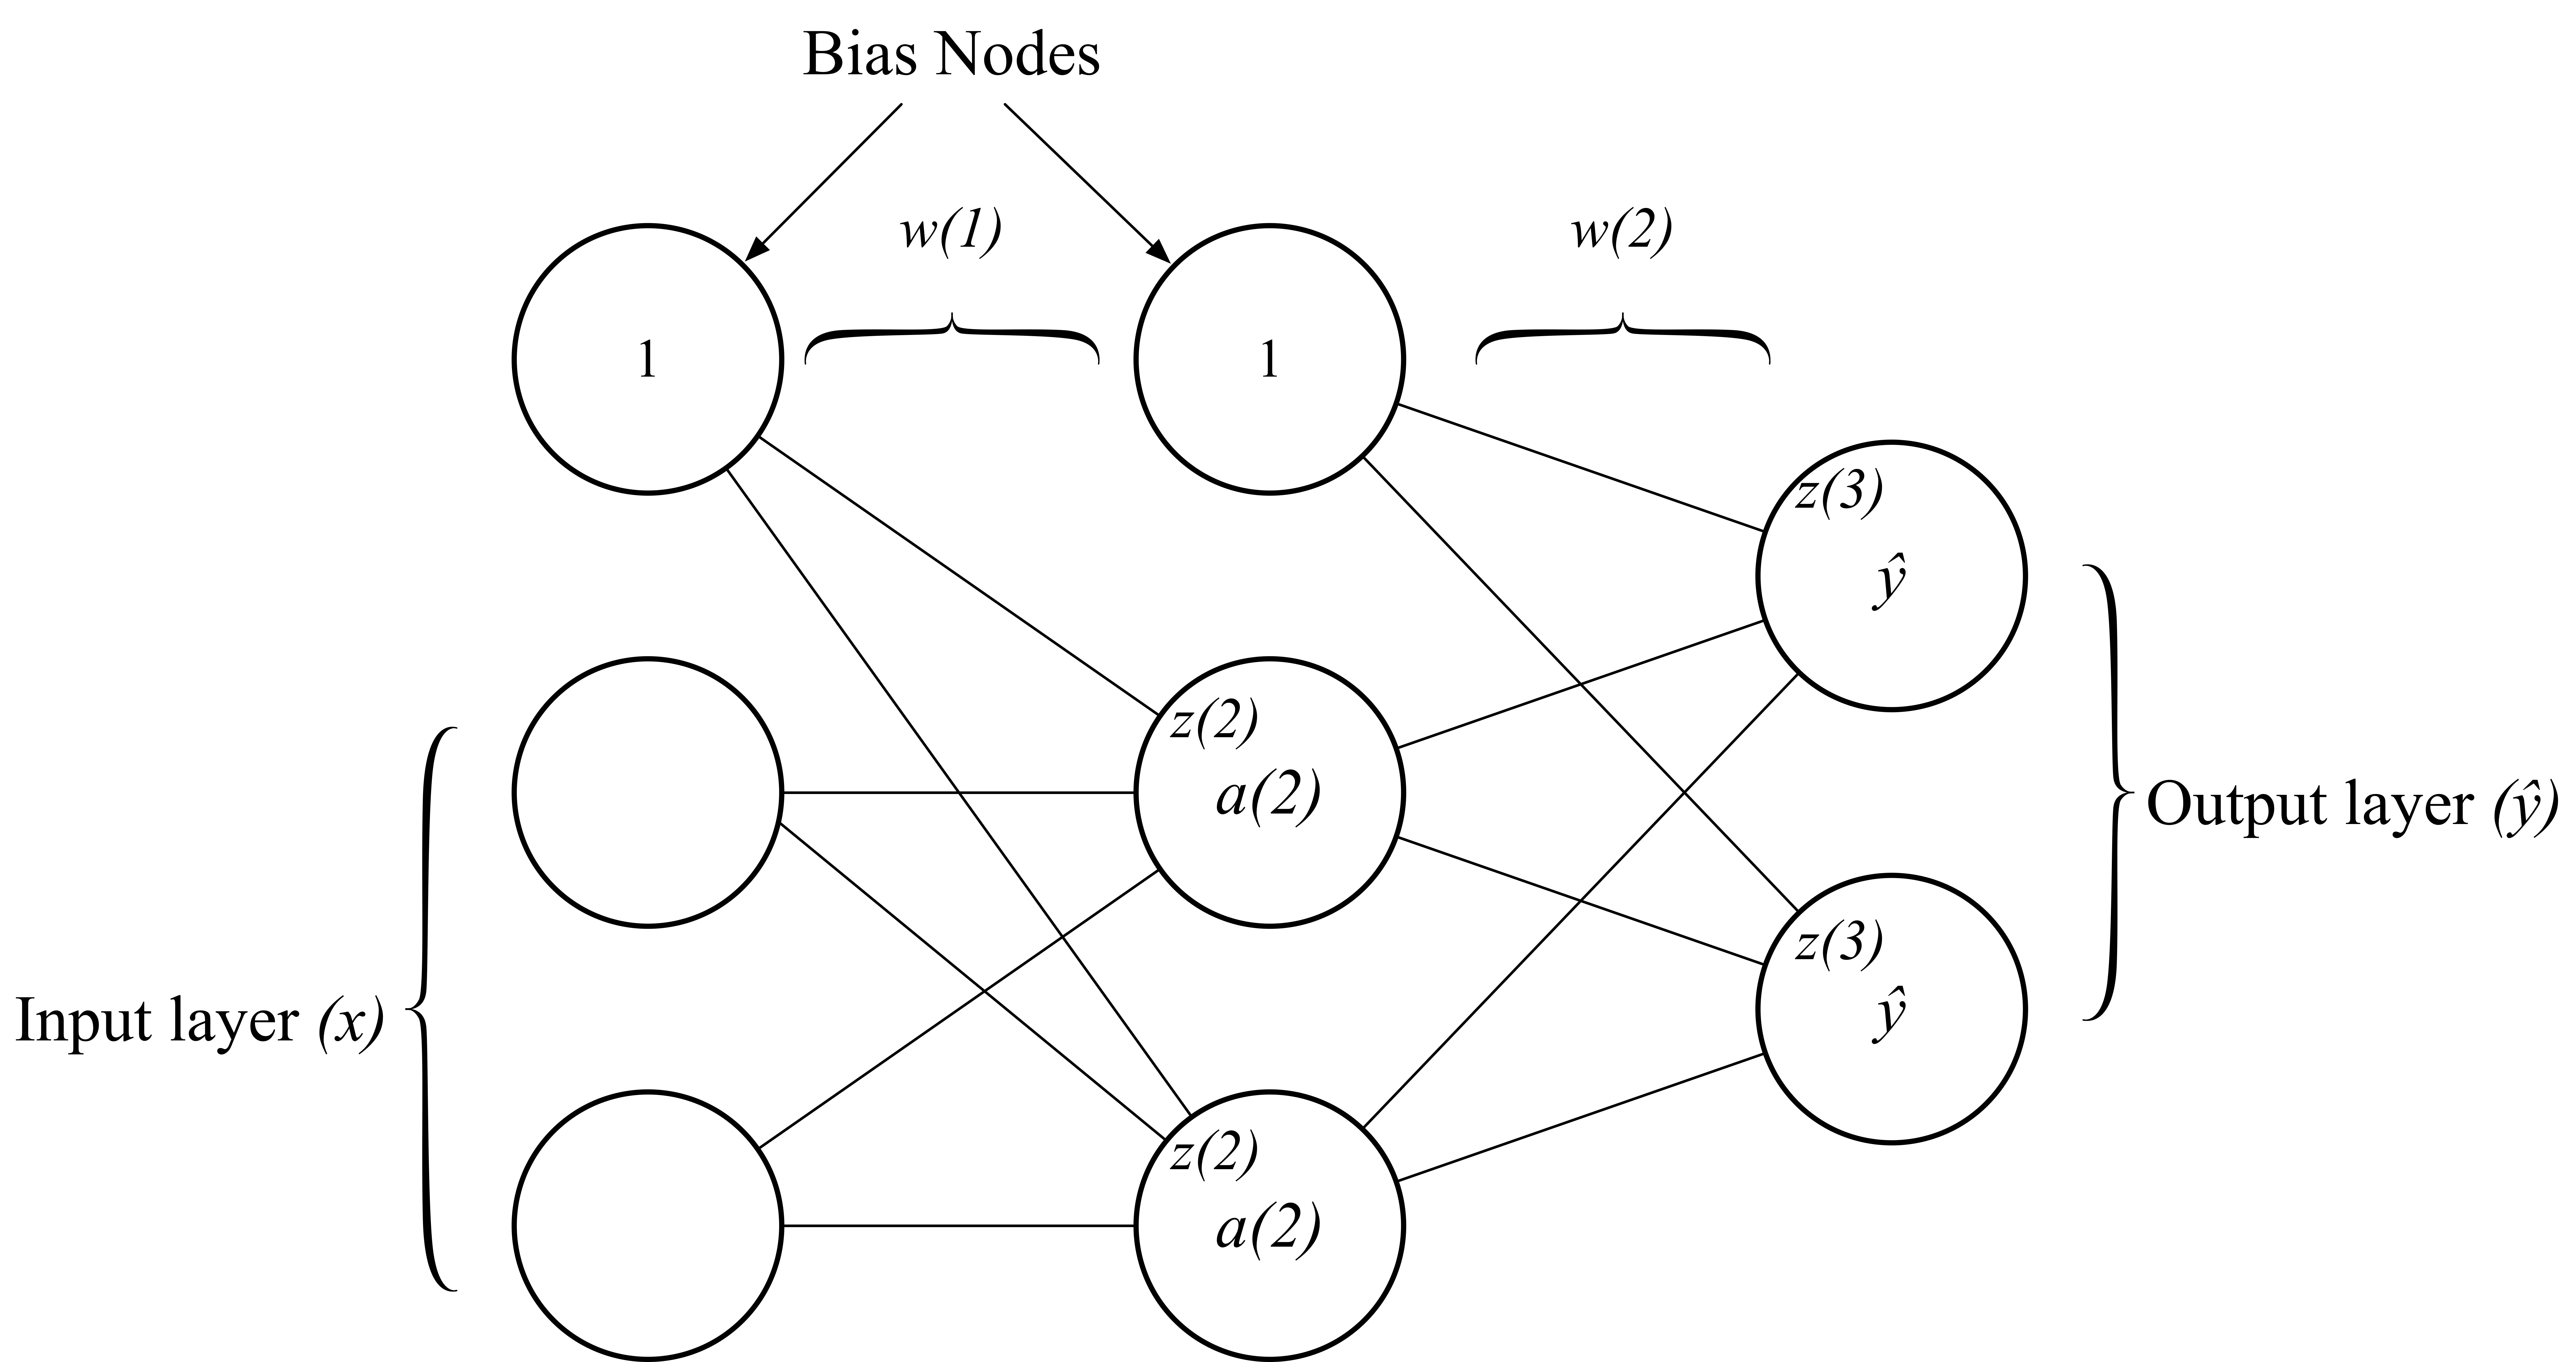
\includegraphics[width=1\linewidth]{nn} }
\centerline{Figure 5}
\vspace{0.5cm}

In a simple three-layer neural network, below are the four equations
that we derive with the principle of gradient descend that will help us
minimize the error.\footnote{The equation was referenced from Michael A. Neilson "Neural Networks and Deep Learning", Determination Press, 2015~}
\[\delta_{(3)} = - (y - \hat{y})(\sigma'(z_{(3)}))\]

Calculate the \(\delta\) for the third layer of the network.
\[\frac{\partial J}{\partial w_{(2)}} = {{(a}^{(2)})}^{T}\delta_{(3)}\]

Use the calculated result to help us modify the second layer of weights
in the network.
\[\delta_{(2)} = \delta_{\left( 3 \right)}\left( w_{\left( 2 \right)} \right)^{T}\sigma'(z_{(2)})\]

Calculate the \(\delta\) for the second layer of the network.
\[\frac{\partial J}{\partial w_{(1)}} = \ x^{T}\delta_{(2)}\]

Finally, we can modify the first layer of weights in the network. This
process is often repeated until the accuracy of the network reaches a
threshold. The backpropagation process above can be represented with this simple diagram of a neural network with one hidden layer. 

\centerline{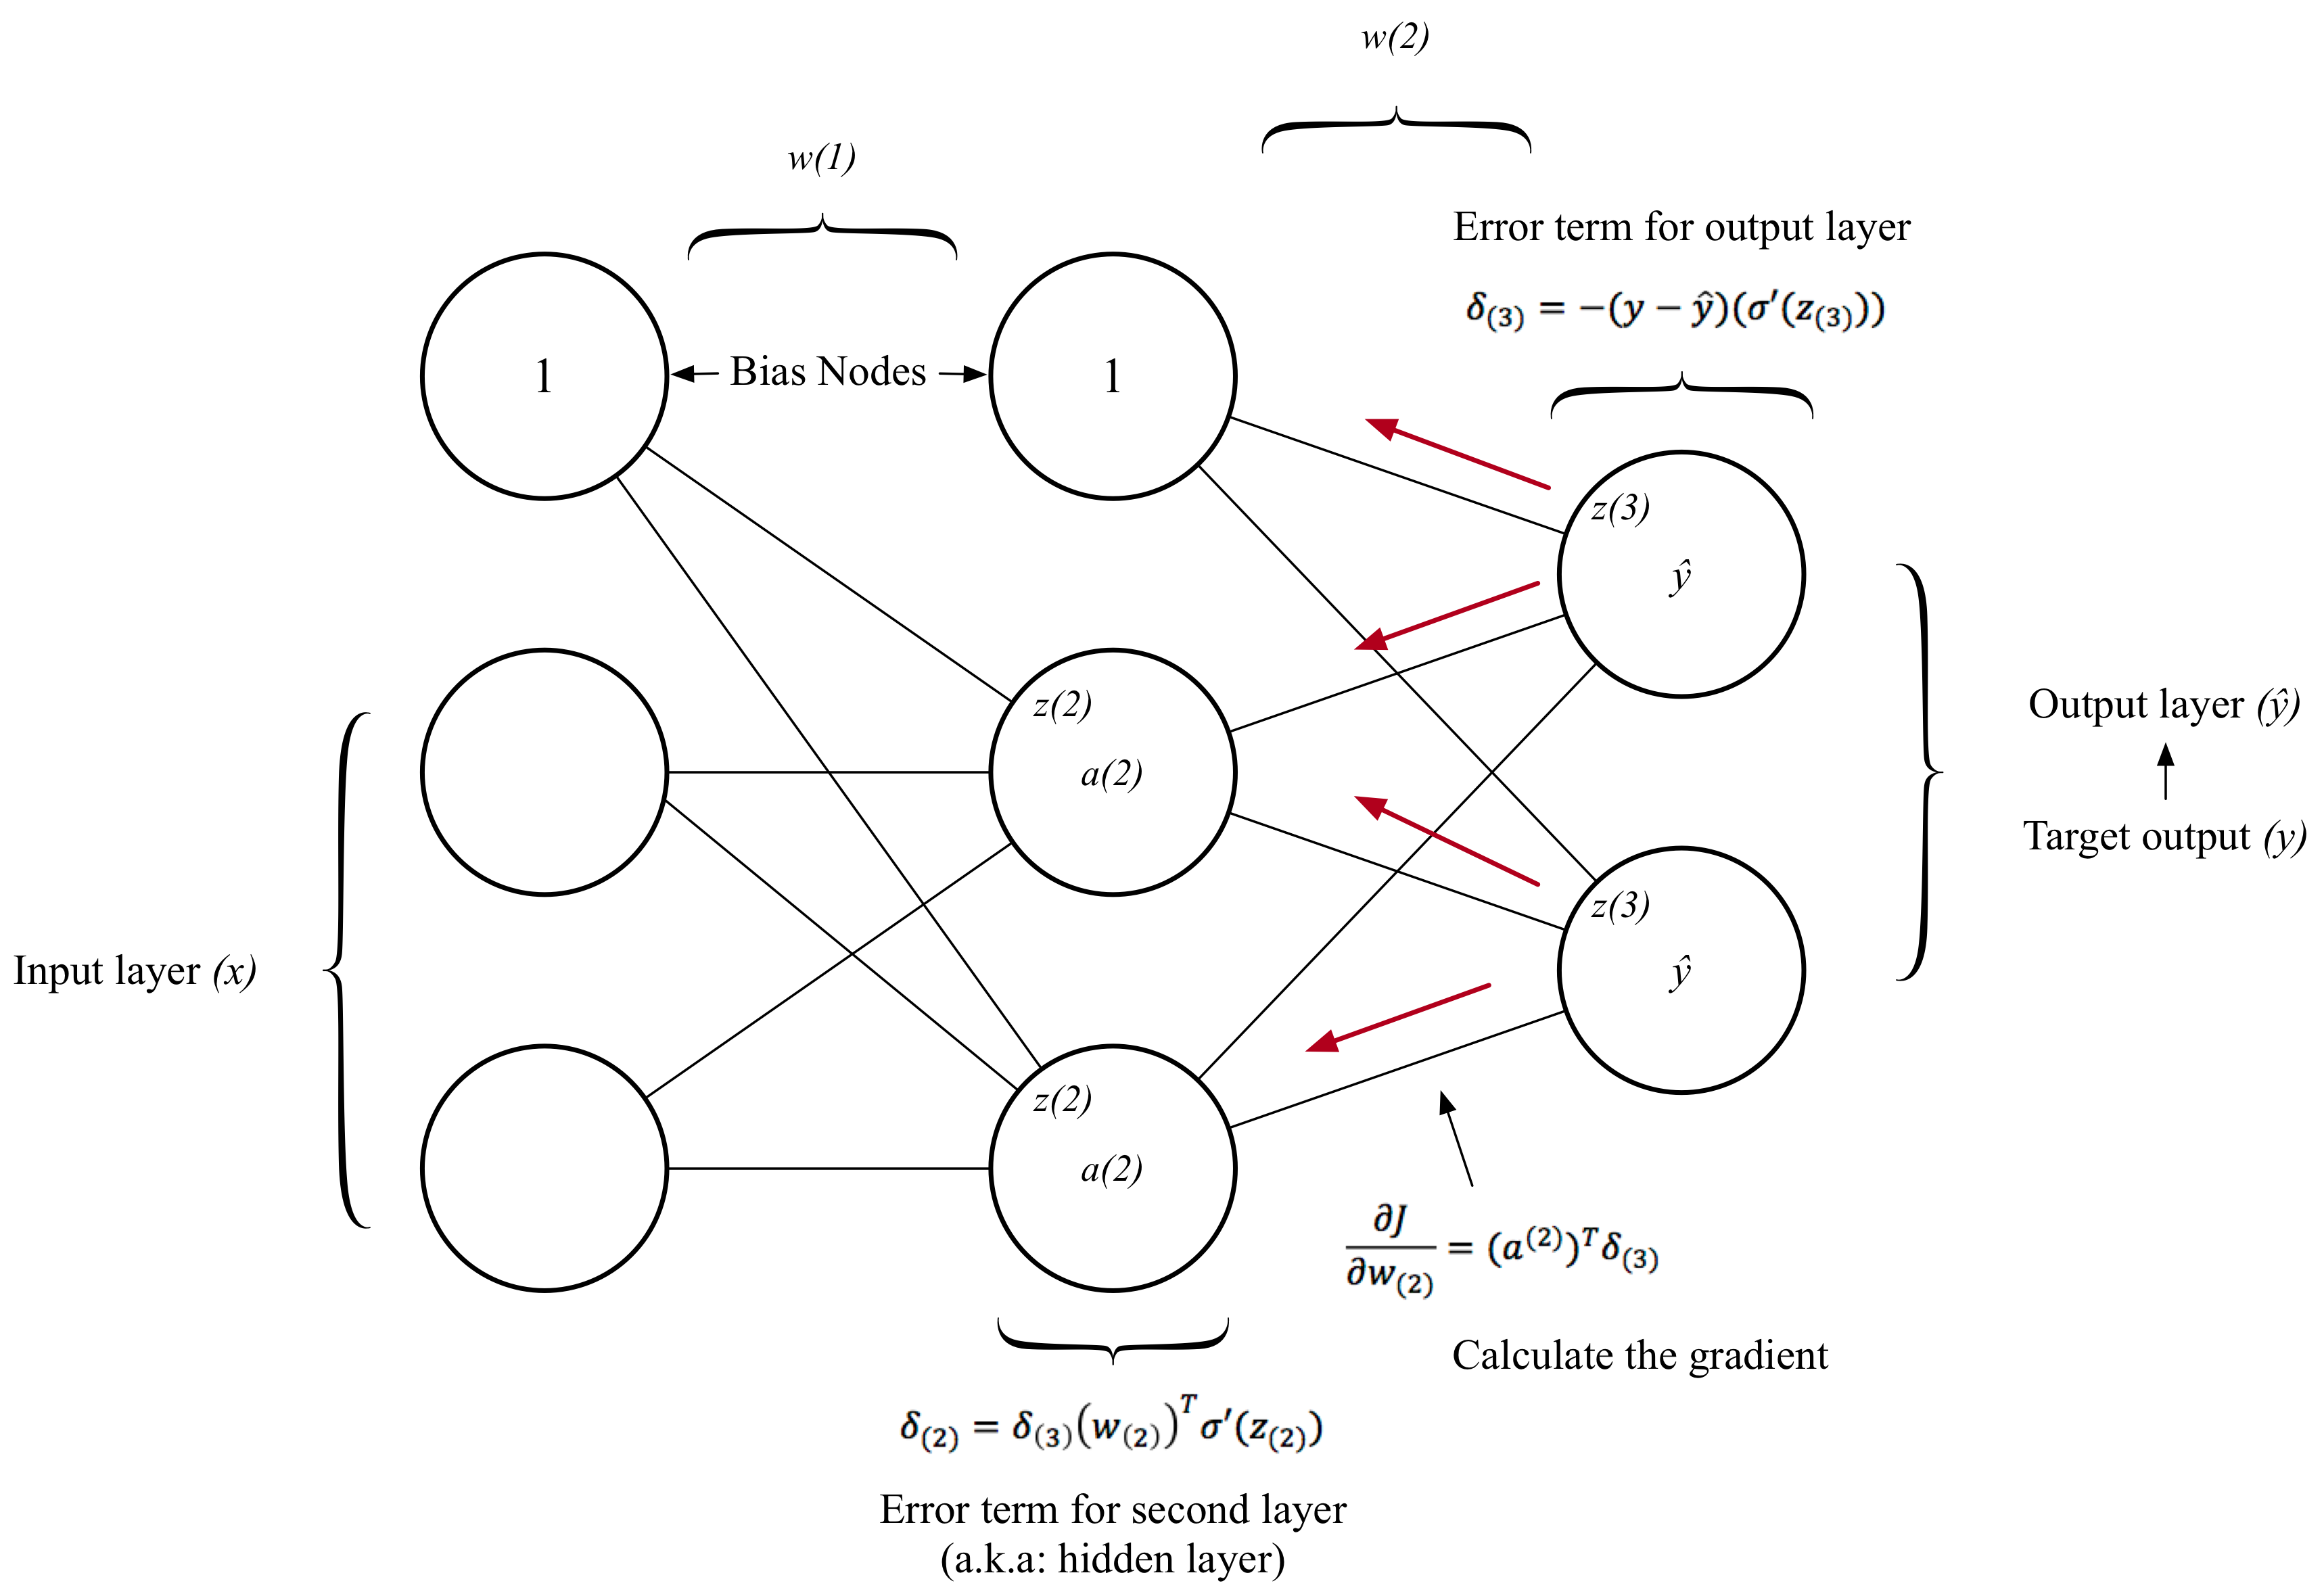
\includegraphics[width=1\linewidth]{nnbp} }
\centerline{Figure 6}
\vspace{0.5cm}

Here is a visualization of how individual output node is approaching the desired output.

\centerline{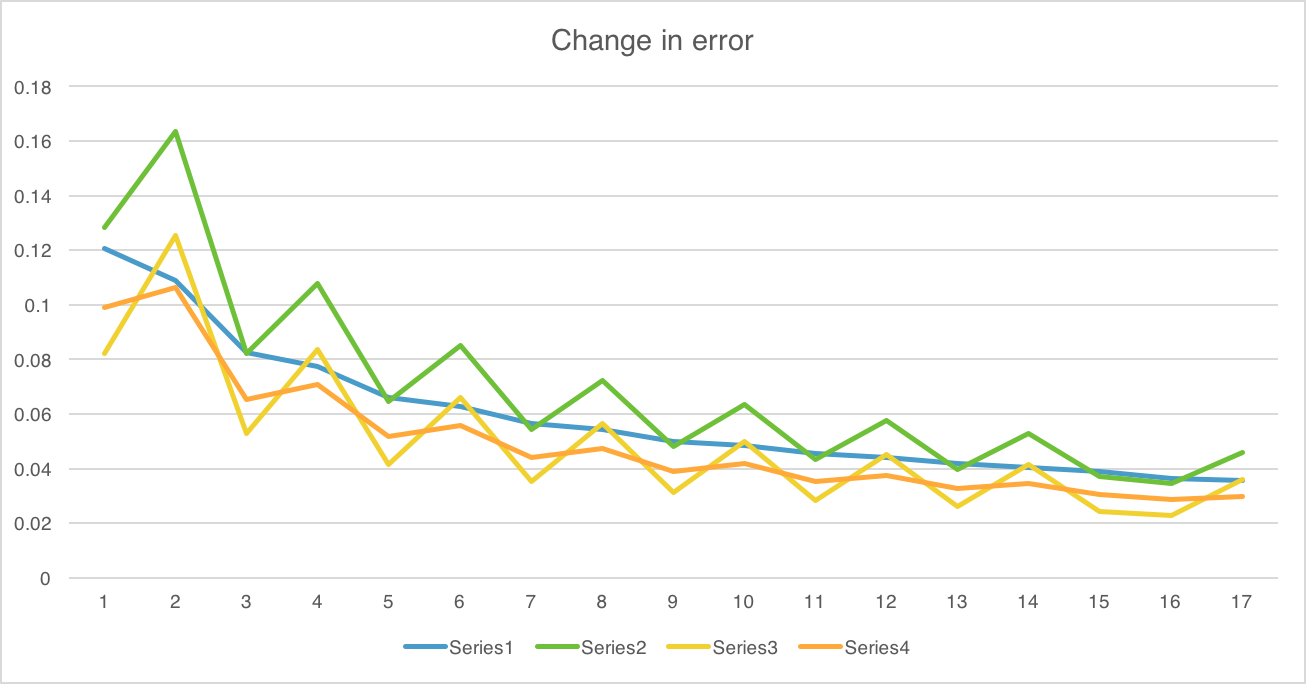
\includegraphics[width=1\linewidth]{graph1} }
\centerline{Figure 7}
\vspace{0.5cm}

Line 0-3 are lowering as we train the network. Line 4, is approaching 1 as we keep train the network. This figure displayed that the error of the network \(C\) is being minimized. 

Here is a graph of the correction of the neural network over times of training. Each time the network will train with 1000 out of 60,000 training data. After, The program will shuffle the training data and repeat the training process for 197 times, or until the network reaches 95\% accuracy. 

\centerline{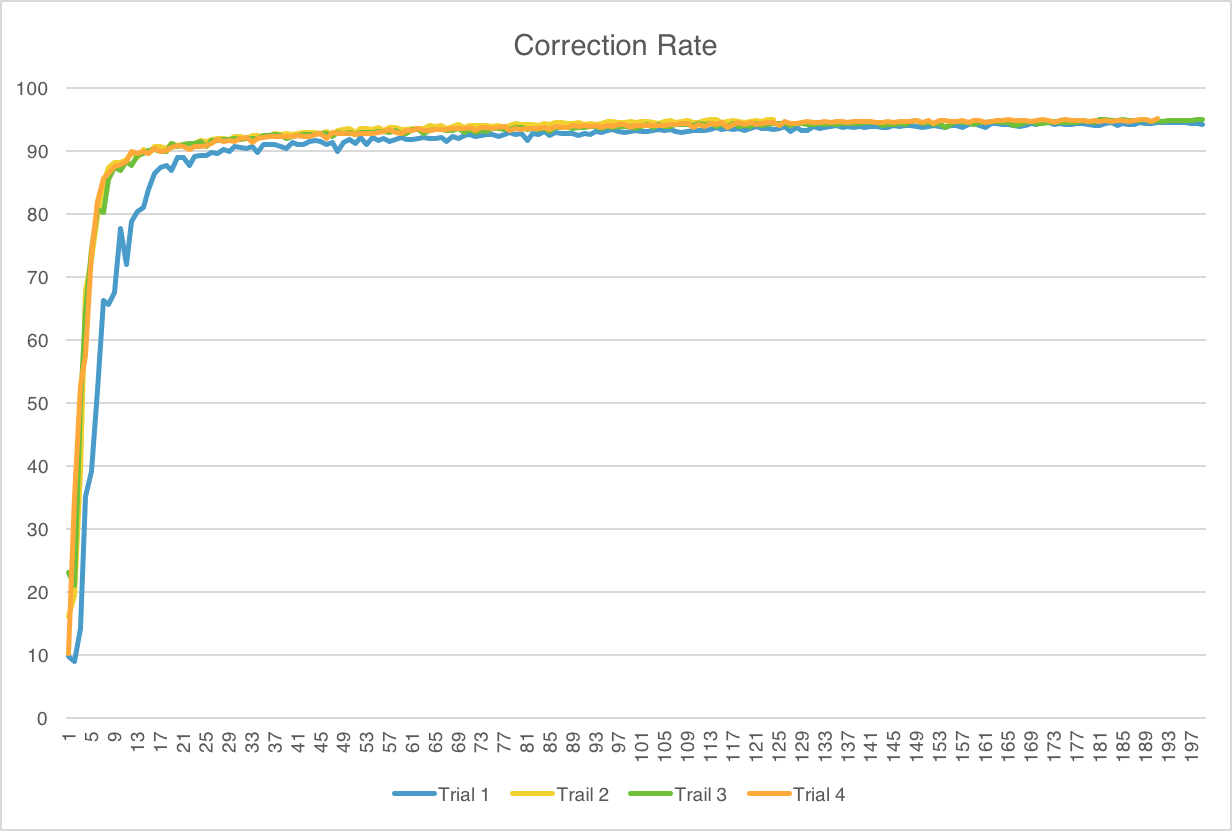
\includegraphics[width=1\linewidth]{graph2}}
\centerline {Figure 8}
\vspace{0.3cm}

The neural network is trained four times with the same training and testing data. The results are similar and the network is steadily improving, thanks to gradient descent. There are many factors that contribute to a successful learning process. If these things are ignored or incorrect, the network will not be able to learn as well. 

%%%%%%%%%%%%%%%%%%%%%%%%%%%%%%%%%%%%%%%%%%%%%%%%%%%%%%%
\section{Improve neural network training result}
Not all neural network behaves flawlessly. Generally, there are a few factors that will effect the training result of the network: hyperparameter, number of hidden nodes, human error, training data/testing data problem and more. Among them, hyperparameter, number of hidden nodes and be determined by estimation and trial and error. Huamn error can be eliminated by debugging. Training data and testing data problem is not easy to solve. That often contributes to the source of your data and the quality of your data, which are beyond the scope of this research. It's safe to assume that the training data and testing data that we are using are carefully chosen and considered.  

\subsection{Making good decision}

In a pre-trained network, there are several critical hyperparameters and numbers that will help the network to improve. I mainly focused on learning rate and number of hidden nodes. 
\subsubsection{Hyperparameters}

Learning rate is the hyperparameter that we will focus on. To make gradient descent work correctly, we need to choose the learning rate \(r\) to be small enough that Equation (9) is a good approximation. If we don't, we might end up with \(\Delta C \textgreater 0\), which will take us to the opposite of minimizing. Meanwhile,  \(r\) can't be too small, since that will make the changes \(\Delta v\) tiny, and thus the gradient descent algorithm will work very slowly. In practical implementations, \(r\) is often varied so that Equation (9) remains a good approximation, but the algorithm isn't too slow. \footnote{Michael A. Nielsen, "Neural Networks and Deep Learning", Determination Press, 2015. \href{http://neuralnetworksanddeeplearning.com/chap1.html}{Chapter 1 Using neural nets to recognize handwritten digits}}

This is a graph of the training result with a different learning rate. The batch size is 1000 and the training is repeated 100 times. 

\centerline{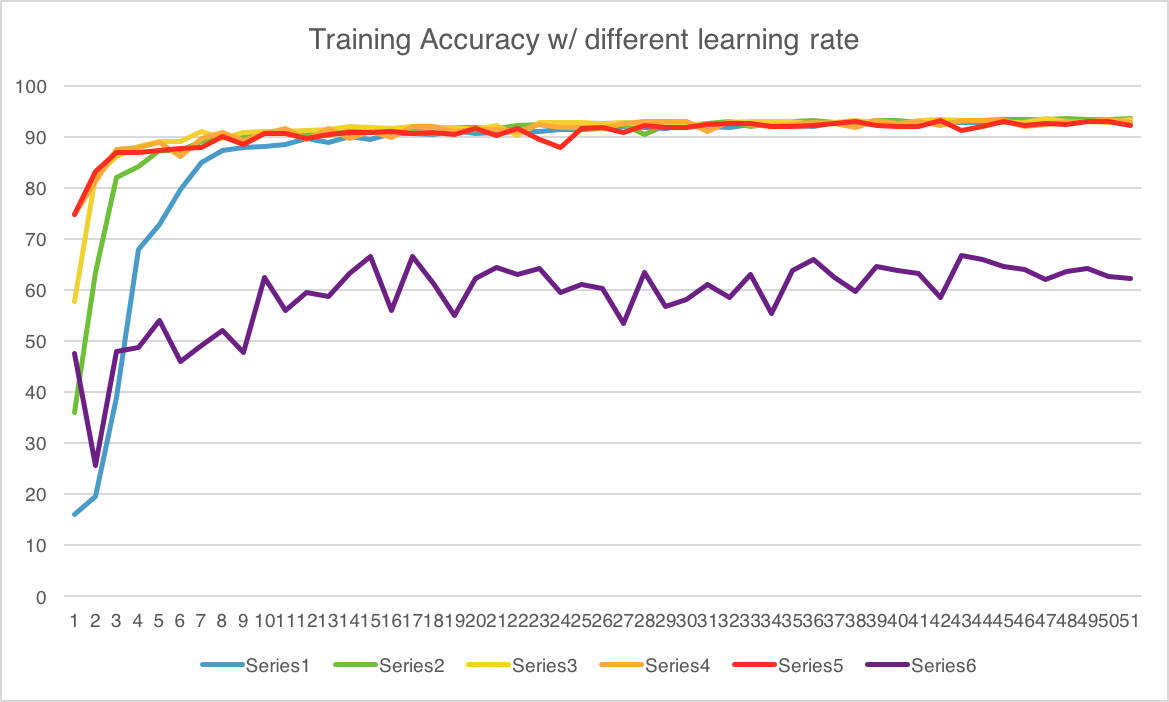
\includegraphics[width=1\linewidth]{graph5}}
\centerline{Figure 9}
\vspace{0.3cm}

The range of the learning rate that I chose is from [0.1, 5]. When the learning rate is relatively low, the network began at a lower accuracy comparing to higher training rates. However, especially when the learning rate is 0.9, the training result became unstable, and the graph starts to oscillate. 

On the other hand, when we set the training rate to 5.0, the network doesn't improve after 40\%-50\%. Then general rule of thumb for choosing the learning rate is somewhere between [0.1-1]. 

With this observation in mind, we might be able to alter the learning rate as the network progress. The training rate should we high in the beginning to quickly bring us to the desired place. Then, we can lower the rate so the network learning result will not have oscillation. 
 
\subsubsection{Hidden nodes}

In a multilayer neural network, you will likely encounter the problem of how many hidden layers and hidden nodes should the network have. Seemingly simple, but complex question will help you improve the learning rate of the network. In this research, we will only focus on one hidden layer. Multiple hidden layer is known as deep learning, which is out of our scope. 

It's difficult to form a good network topology just from the number of inputs and outputs. It depends critically on the number of training examples and the complexity of the classification you are trying to learn. There are problems with one input and one output that require millions of hidden units, and problems with a million inputs and a million outputs that require only one hidden unit, or none at all.

Below if a graph of a neural network with different number of hidden nodes. There is a healthy range of number of hidden nodes. If there is one hidden node, the accuracy will not be more than 25\% and also defeat the purpose of the neural network. If there are too many nodes, calculation becomes gruesome and the accuracy is similar to lower number of nodes. Therefore, the number of hidden nodes highly depend your data, network, situation and needs. 

\centerline{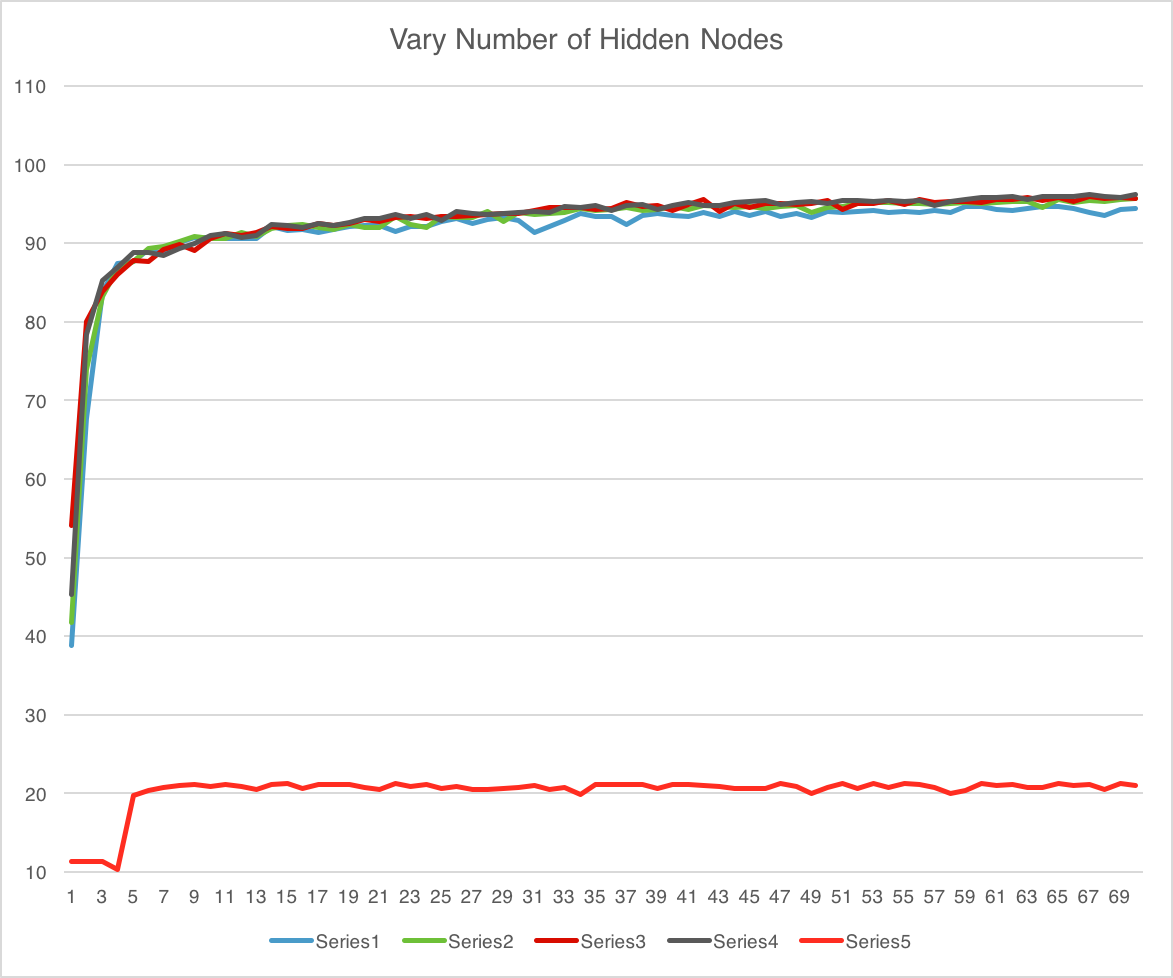
\includegraphics[width=1\linewidth]{graph6}}
\centerline{Figure 10}
\vspace{0.5cm}

\subsection{Improve training result with dynamic hyperparameter}

In section 7.1.1, I stated that the learning rate will effect how the network learns in the beginning. Higher learning rate means that it will start at a higher success rate and gradually improve. However, high learning rate will lead to noticeable fluctuations in the learning rate. This observation gives us the possibility to change the learning rate as the network learns. In the beginning, we will set the learning rate 0.8, then slowly lower the the learning rate as the network improves. 

This concept will seem intuitive in that you want the network slow down the learning rate when it's close to the desired result. Otherwise, a high learning rate will likely create some fluctuation like we have seen figure 2. 

Below is a accuracy graph of a neural network with 0.8 learning rate. The network is trained with batches of 1000 data and shuffled before the next training. Training is stopped after the accuracy on test data reaches 95\%. All of its hyparameters were static during training. 

\centerline{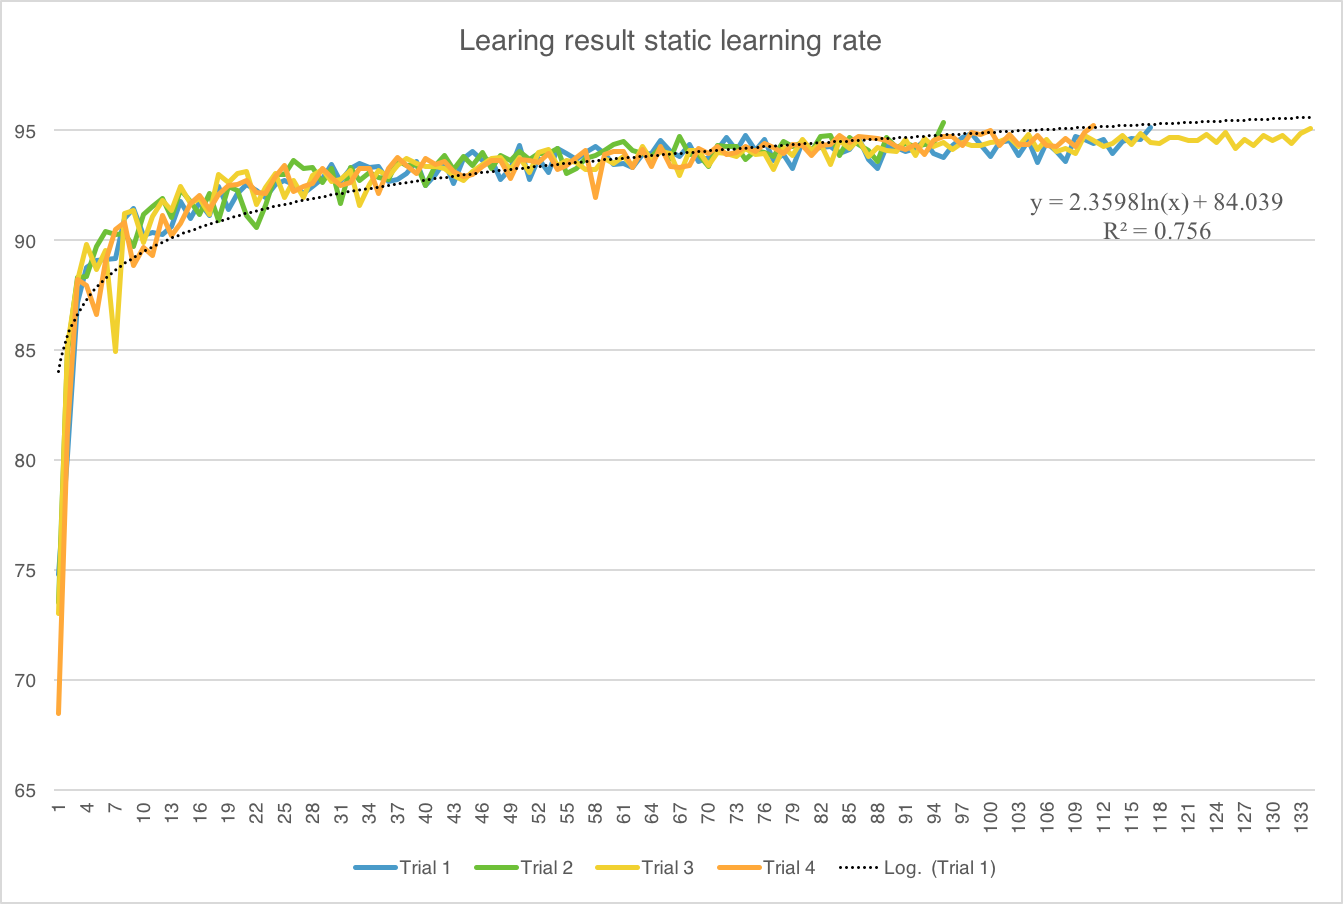
\includegraphics[width=1\linewidth]{graph7} }
\centerline{Figure 11}
\vspace{0.5cm}

The training time is mediocre comparing to a well optimized network. The average training time is around 360 second and the number of epoch is around 110. In another word, the network took 6 minutes and 12,000 data to reach 95\% accuracy. 

We can improve this result by lowering the learning rate of the network as it improves. Specially, the network begins to lower the learning rate when the accuracy reaches 93\%. The new accuracy is calculated by 

\begin{equation}
	r_{(new)} = r_{(old)} * 0.9\
\end{equation}

Once again, the network is trained with batches of 1000 data and shuffled before the next training. Training is stopped after the accuracy on test data reaches 95\%.

\centerline{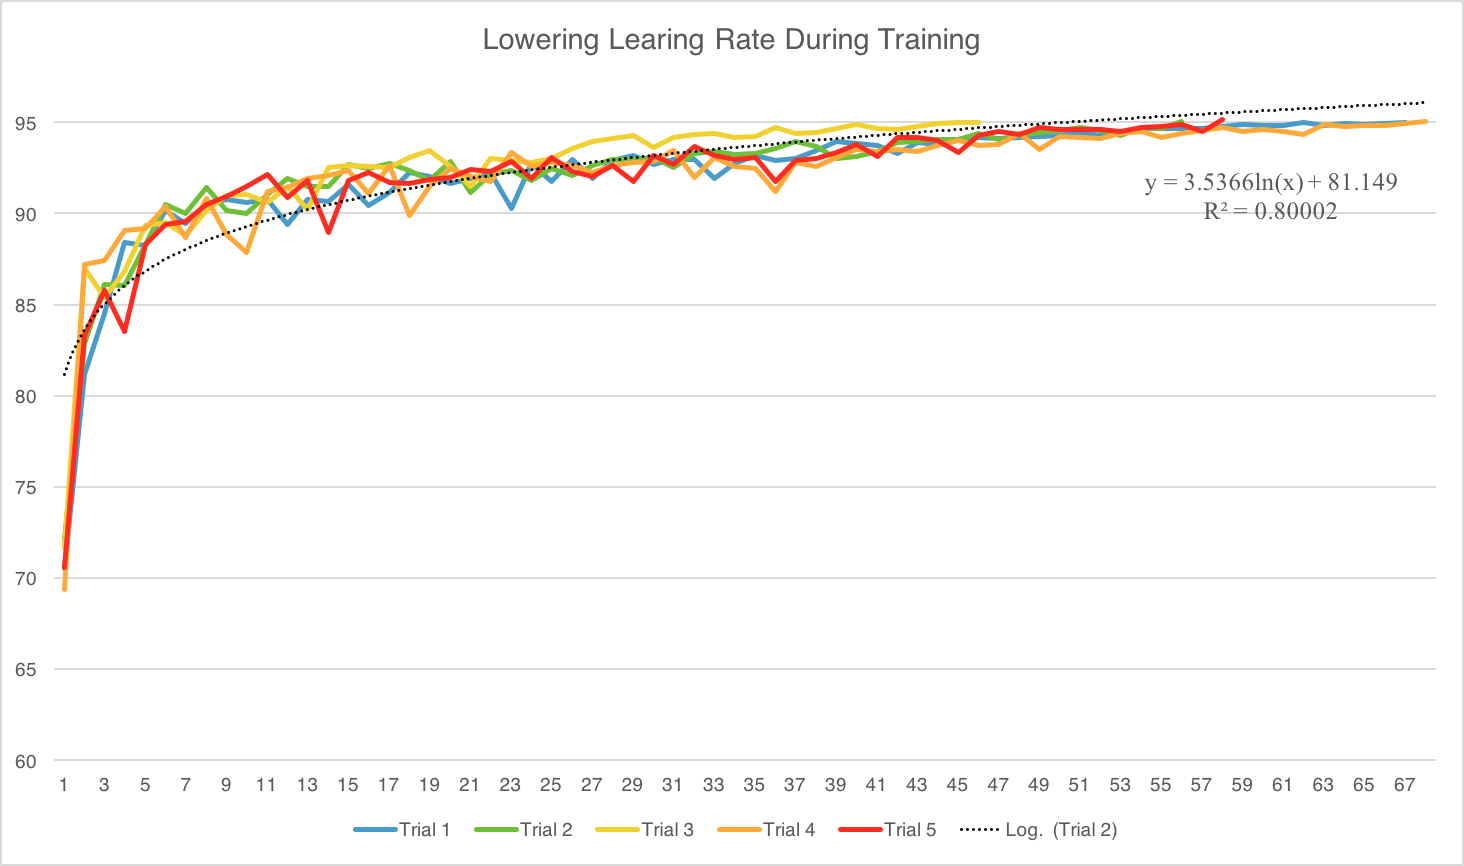
\includegraphics[width=1\linewidth]{graph8} }
\centerline{Figure 12}
\vspace{0.5cm}

Clearly, the network took much less time and epoch to reach 95\%. 
\centerline{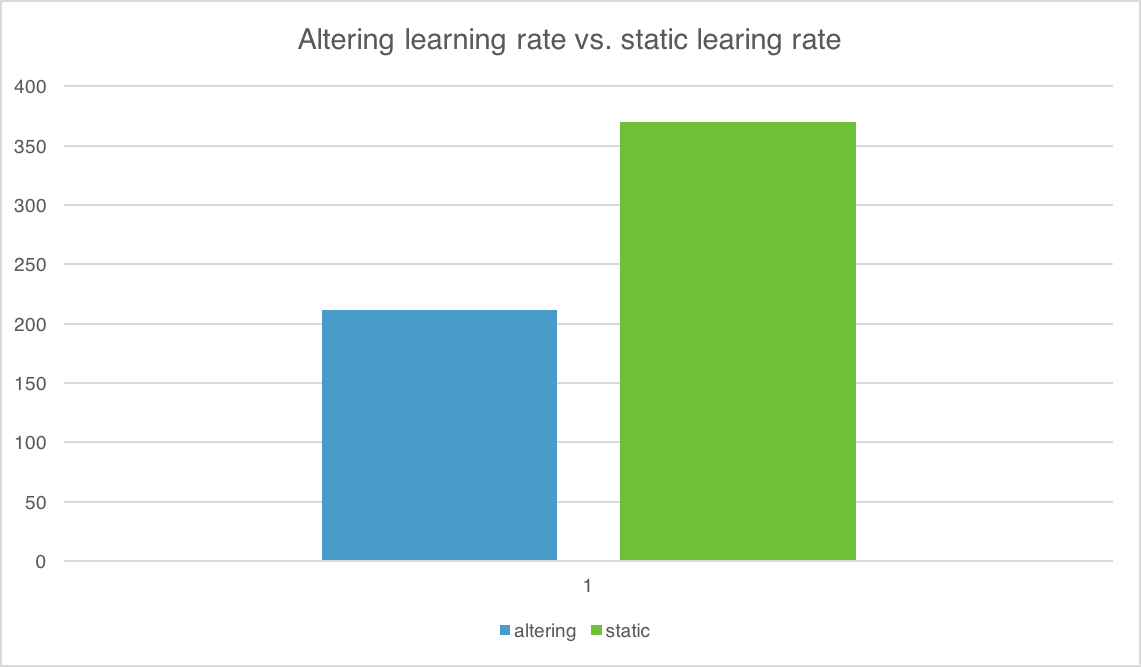
\includegraphics[width=1\linewidth]{graph10} }
\centerline{Figure 13}
\vspace{0.5cm}

The training time difference between dynamic and static learning rate is more than 300 seconds. 

\centerline{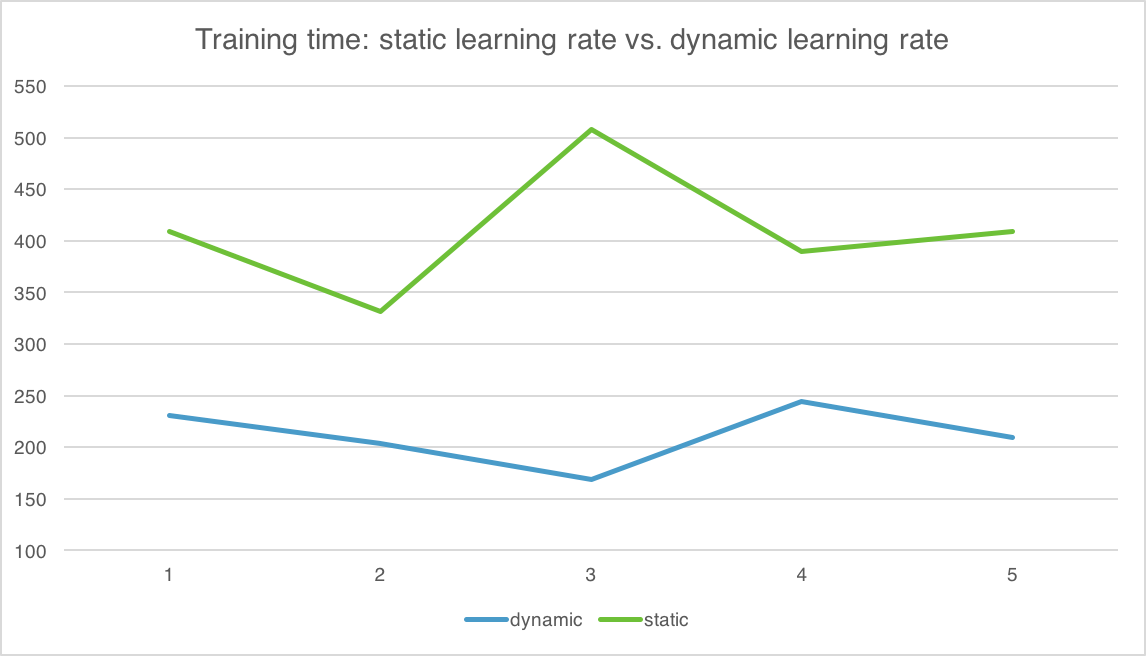
\includegraphics[width=1\linewidth]{graph11} }
\centerline{Figure 14}
\vspace{0.5cm}

Comparing two results, we can calculate a LBF (line of best fit) for the accuracy rate. By comparing the two \(ln\) functions, the function in Figure (12) has a higher coefficient, which means that the growth of the curve will be greater. In another word, by adjusting the learning rate, the network was able to learn more quickly and efficiently. 

\section{Future studies}

Finally, you have made it to the end. Thank you for staying with me throughout the paper. I hope you find neural networks amazing. It will bring tremendous change and power to computing technologies. The current computing power is far from simulating a biological brain. However, our understanding of it has helped us to develop technologies such as neural network and deep learning. 

Specifically, in this research, I only touched the surface of neural networks. The field is enormous and requires all types of scientist to improve it. I avoided topics such as: different types of activation functions, some mathematical proves, details on improving neural network and finally, deep learning. Further development in the areas above will enhance current technologies and open doors to new opportunities. 

In fact, many of my dedicated friends and colleges are working on these hard problems. Mr. Meng focused deeply on the mathematics behind neural networks. Mr. McAvoy developed other learning algorithms. In the larger realm, Google DeepMind is trying to create a comprehensive A.I. system; Google translate team made important breakthroughs in 2016 on their multilingual neural machine translation system. 

Thank you again for taking your time to read this paper. I hope you are also excited to jump into the field and be apart of this great journey of studying, developing and exploring the world of machine learning, and eventually artificial intelligence. 

\end{multicols}

\end{document}
